%epidemic limitado, entrega directa
\subsubsection{Spray-and-Wait}
Spray-and-Wait\cite{sandw} es un protocolo que realiza forward y entrega directa, en dos fases distintas. El nodo de origen genera L copias, que esparce según cierta distribución. Normalmente se utiliza spray binario, es decir, cada nodo reparte la mitad de sus copias al nodo que encuentra, esperando que éste a su vez entregue la mitad al topar un nuevo nodo que no tenga el mensaje, como se ve en la Figura \ref{fig:hpa}; o spray directo, donde sólo el nodo de origen reparte 1 copia a cada nodo que ve. Al terminar el spray, es decir, cuando cada nodo cuenta con sólo una copia, si no se encontró al destinatario en esa fase, se pasa a esperar, donde cada nodo intenta entregar el mensaje directamente al nodo final.
Spray-and-Wait obtiene mejores resultados que los protocolos de \emph{flooding}.

\begin{figure}[h]
\centering
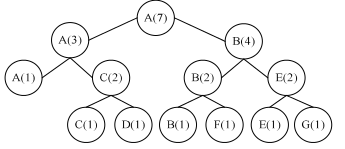
\includegraphics[width=200px]{HPA.png}
\caption{Spray Binario \cite{crhc}}
\label{fig:hpa}
\end{figure}